\documentclass[a4paper, 10pt]{article}
\usepackage{helvet}
\renewcommand{\familydefault}{\sfdefault}
\usepackage{pgf}
\usepackage{eurosym}
\usepackage{graphicx}
\usepackage{wasysym}
\usepackage{hyperref}
\usepackage{listings}
\usepackage{pxfonts}
\usepackage{verbatim}
\usepackage{color}
\usepackage{xcolor}
\usepackage{wrapfig}
\usepackage{enumitem}
\usepackage{booktabs}
\usepackage{gensymb}
\usepackage{tabularx}
\usepackage{currfile}

\hypersetup{
    bookmarks=true,         % show bookmarks bar?
    unicode=true,          % non-Latin characters in Acrobat’s bookmarks
    pdftoolbar=true,        % show Acrobat’s toolbar?
    pdfmenubar=true,        % show Acrobat’s menu?
    pdffitwindow=true,     % window fit to page when opened
    pdftitle={Assessments},    % title
    pdfauthor={Paul Vesey},     % author
    pdfsubject={Building Information Modelling },   % subject of the document
    pdfcreator={},   % creator of the document
    pdfproducer={xelatex}, % producer of the document
    pdfkeywords={'Graphics' }, % list of keywords
    pdfnewwindow=true,      % links in new PDF window
    colorlinks=true,       % false: boxed links; true: colored links
    linkcolor=violet,          % color of internal links (change box color with linkbordercolor)
    citecolor=magenta,        % color of links to bibliography
    filecolor=red,      % color of file links
    urlcolor=blue           % color of external links
}

\setlength\parindent{0pt}
\begin{document}

\lstset{language=HTML,
				basicstyle=\small,
				breaklines=true,
        numbers=left,
        numberstyle=\tiny,
        showstringspaces=false,
        aboveskip=-20pt,
        frame=leftline
        }
				
\begin{figure}
	\centering
	
\includegraphics[width=0.5\linewidth]{./Assignments/img/LITlogo}
\end{figure}


\begin{tabularx}{\textwidth}{ |l|X| }
	\hline
	\textbf{Subject:} & Revit MEP\\
	\textbf{Course:} & Building Information Modelling with Revit MEP\\
	\textbf{Session:} & Autumn 2021\\
	\textbf{Lecturer:} & Paul Vesey \footnotesize{BEng, MIE, HDip}\\
	\textbf{Filename:} & \currfilebase\\
	\hline
\end{tabularx}



\vspace{0.25cm}	
	
\part*{Assignment 1 (33\%) - Detached 2 Storey Residence with Dormer Window}

\begin{tabularx}{\textwidth}{ |X|X| }
	\hline
	\textbf{Issue Date:} & As stated on Moodle \\
	\hline 
	\textbf{Submission Date:}  & As stated on Moodle  \\
	\hline
\end{tabularx}


\section*{Assignment Outline}


You are required to model a two storey house incorporating a dormer window and to digitally submit you project file (.rvt) showing your model on one A4 sheet and three A1 sheets.


\section*{Your Submission should contain the following drawings}



\begin{tabularx}{\textwidth}{ |c|c|X| }
	\hline
	\textbf{Sheet Size} & \textbf{Sheet No.} & \textbf{Title} \\
	\hline 
	A4  & A101 & Cover Sheet \\
	A1  & A102 & Floor Plans \\
	A1  & A103 & Elevations \\
	A1  & A104 & Sections and Details \\
	\hline
\end{tabularx}

Details of the requirements for each drawing are given below:\\

\subsection*{A101 - Cover Sheet}
\begin{itemize}
	\item Three Dimensional (Aerial View) of the model (scaled to suit the sheet size) Shaded
	\item A list of the drawings in the design pack
\end{itemize}


\subsection*{A102 - Floor Plans}
\begin{itemize}
	\item Ground and First Floor Plans @ 1:50 with dimensions, Room Titles ans some fixed furniture
	\item Two internal camera views, (scaled to suit the sheet size) rendered using the Autodesk 360 cloud rendering service.  \textit{One of the fireplace and one of the kitchen units} 
\end{itemize}


\subsection*{A103 - Elevations}
\begin{itemize}
	\item South Elevation @ 1:50
	\item North, East and West Elevations @ 1:100
\end{itemize}

\subsection*{A104 - Sections and Details}
\begin{itemize}
	\item Three sections are required
	\item Section thro' Kitchen / Sitting Room facing East (towards fireplace) @ 1:100
	\item Section thro' Kitchen / Sitting Room facing West (towards kitchen units) @ 1:100
	\item Section thro' the Hallway / Landing showing the Stairs and the Dormer @ 1:100
	\item One full height detail (Call-outs) @ 1:20, including Repeating Details showing the following:
	\begin{itemize}
		\item Foundation / External Wall / Floor Interfaces
		\item Facia / Soffit and Roof Details
		\item All necessary notes
	\end{itemize} 
\end{itemize}

Additional Sheets may be submitted if so desired.


\begin{flushleft}
\section*{Presentation and Submission}
\end{flushleft}


\begin{enumerate}
	\item All drawing sheets must have the LIT Built Environment logo and be clearly marked 'Educational Exercise - Not for Construction'
	\item You are required to submit you project as a single Revit (.rvt) file through Moodle
	\item Drawings should show all necessary information to communicate design intent
	\item The Revit filename should be of the form \textit{Semester  + Year + Project No. + First Initial + Surname + K-Number}. An example would be \textbf{'Spring18P01PVeseyK00123456.rvt'}.  Do not use spaces in the filename
\end{enumerate}


\newpage

\section*{Design Specification}



The total floor area of the house should be approx 150$m^2$\\

The following design may be used as a guide.  You may modify the proportions provided you maintain a protrusion at the front of the building.


\begin{itemize}
	\item Enterance Hall (2400mm wide)
	\item Universilly Accessible Bathroom / Toilet
	\item Kitchen / Dining (with fixed and loose furniture)
	\item Living Room / Sitting Room (with direct access to kitchen)
	\item Ground Floor Bedroom (Playroom / Study)
	\item Externally accessed boiler house/shed
	\item Stairs 900mm wide (Rise 171.9mm, Going 280mm)
\end{itemize}



\begin{figure}
	\centering
	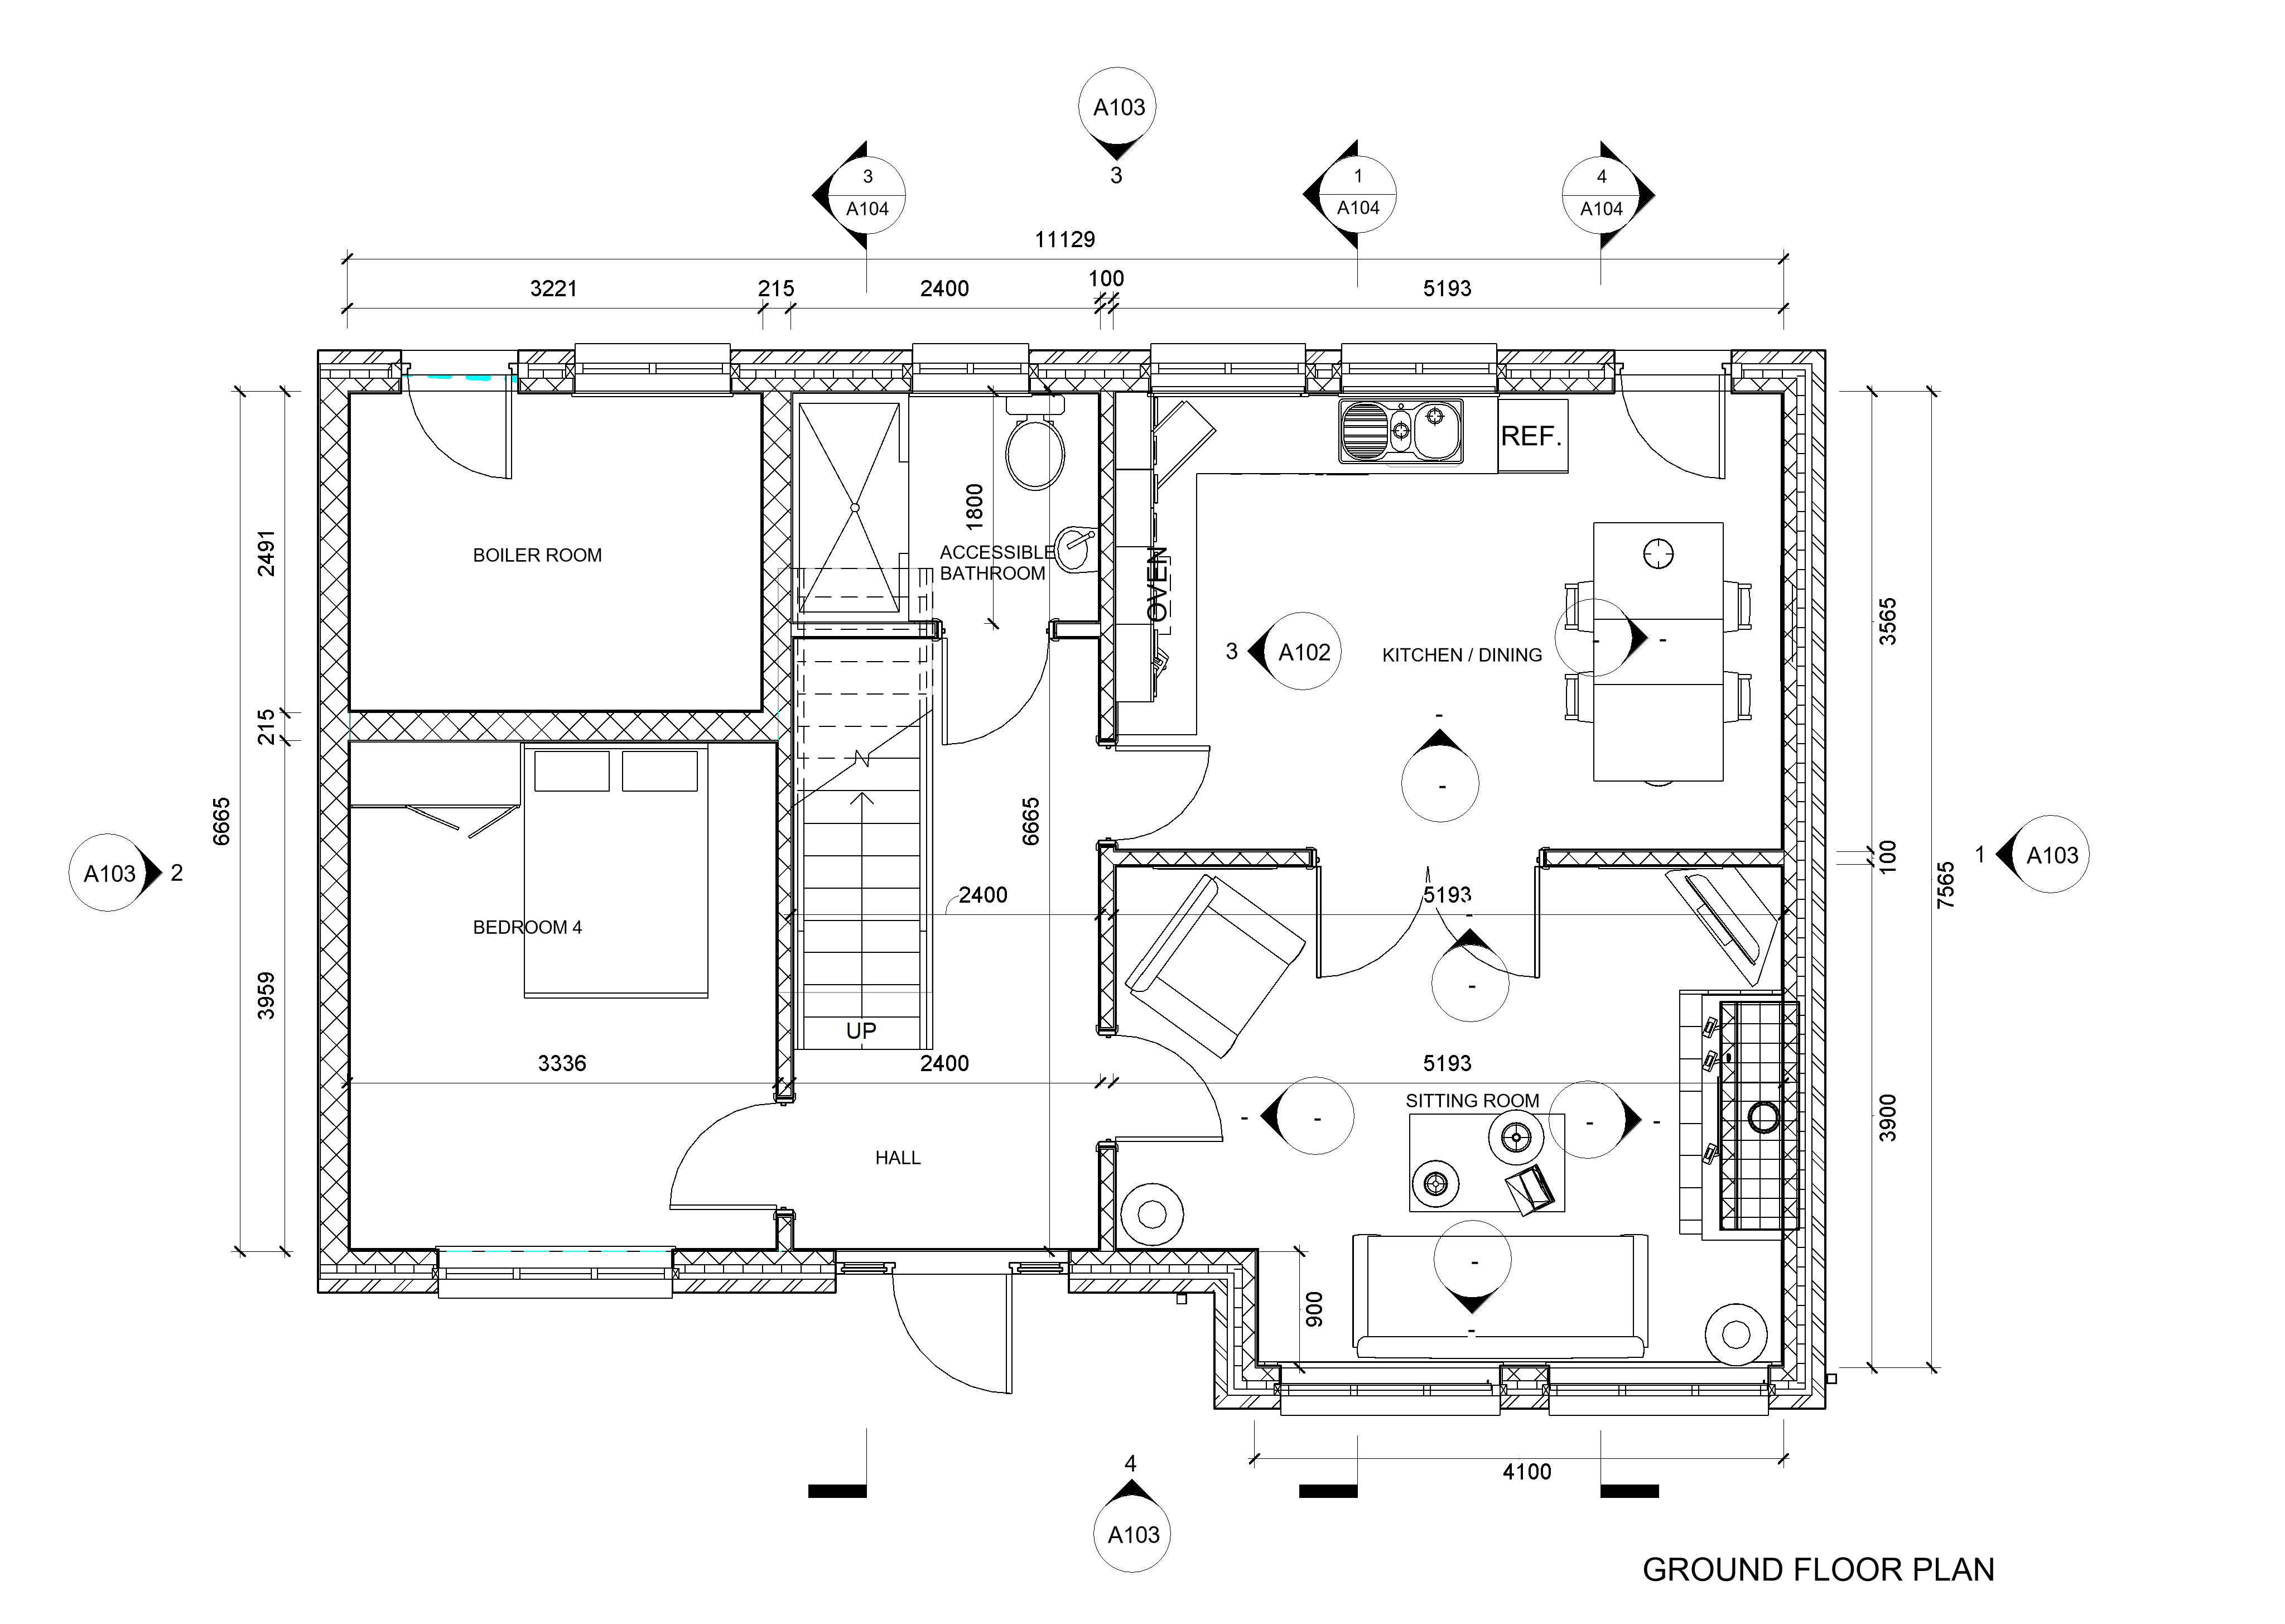
\includegraphics[width=1.0\linewidth]{img/P01GroundFloorLevel.jpg}
	\caption{Ground Floor}
	\label{fig:p01groundfloorlevel}
\end{figure}


\newpage

\begin{itemize}
	\item 3 Bedrooms with en-suite sanitary facilities
	\item Main Bathroom with Bath or Shower, WC and sink
	\item Hot Press
\end{itemize}



\begin{figure}[th]
	\centering
	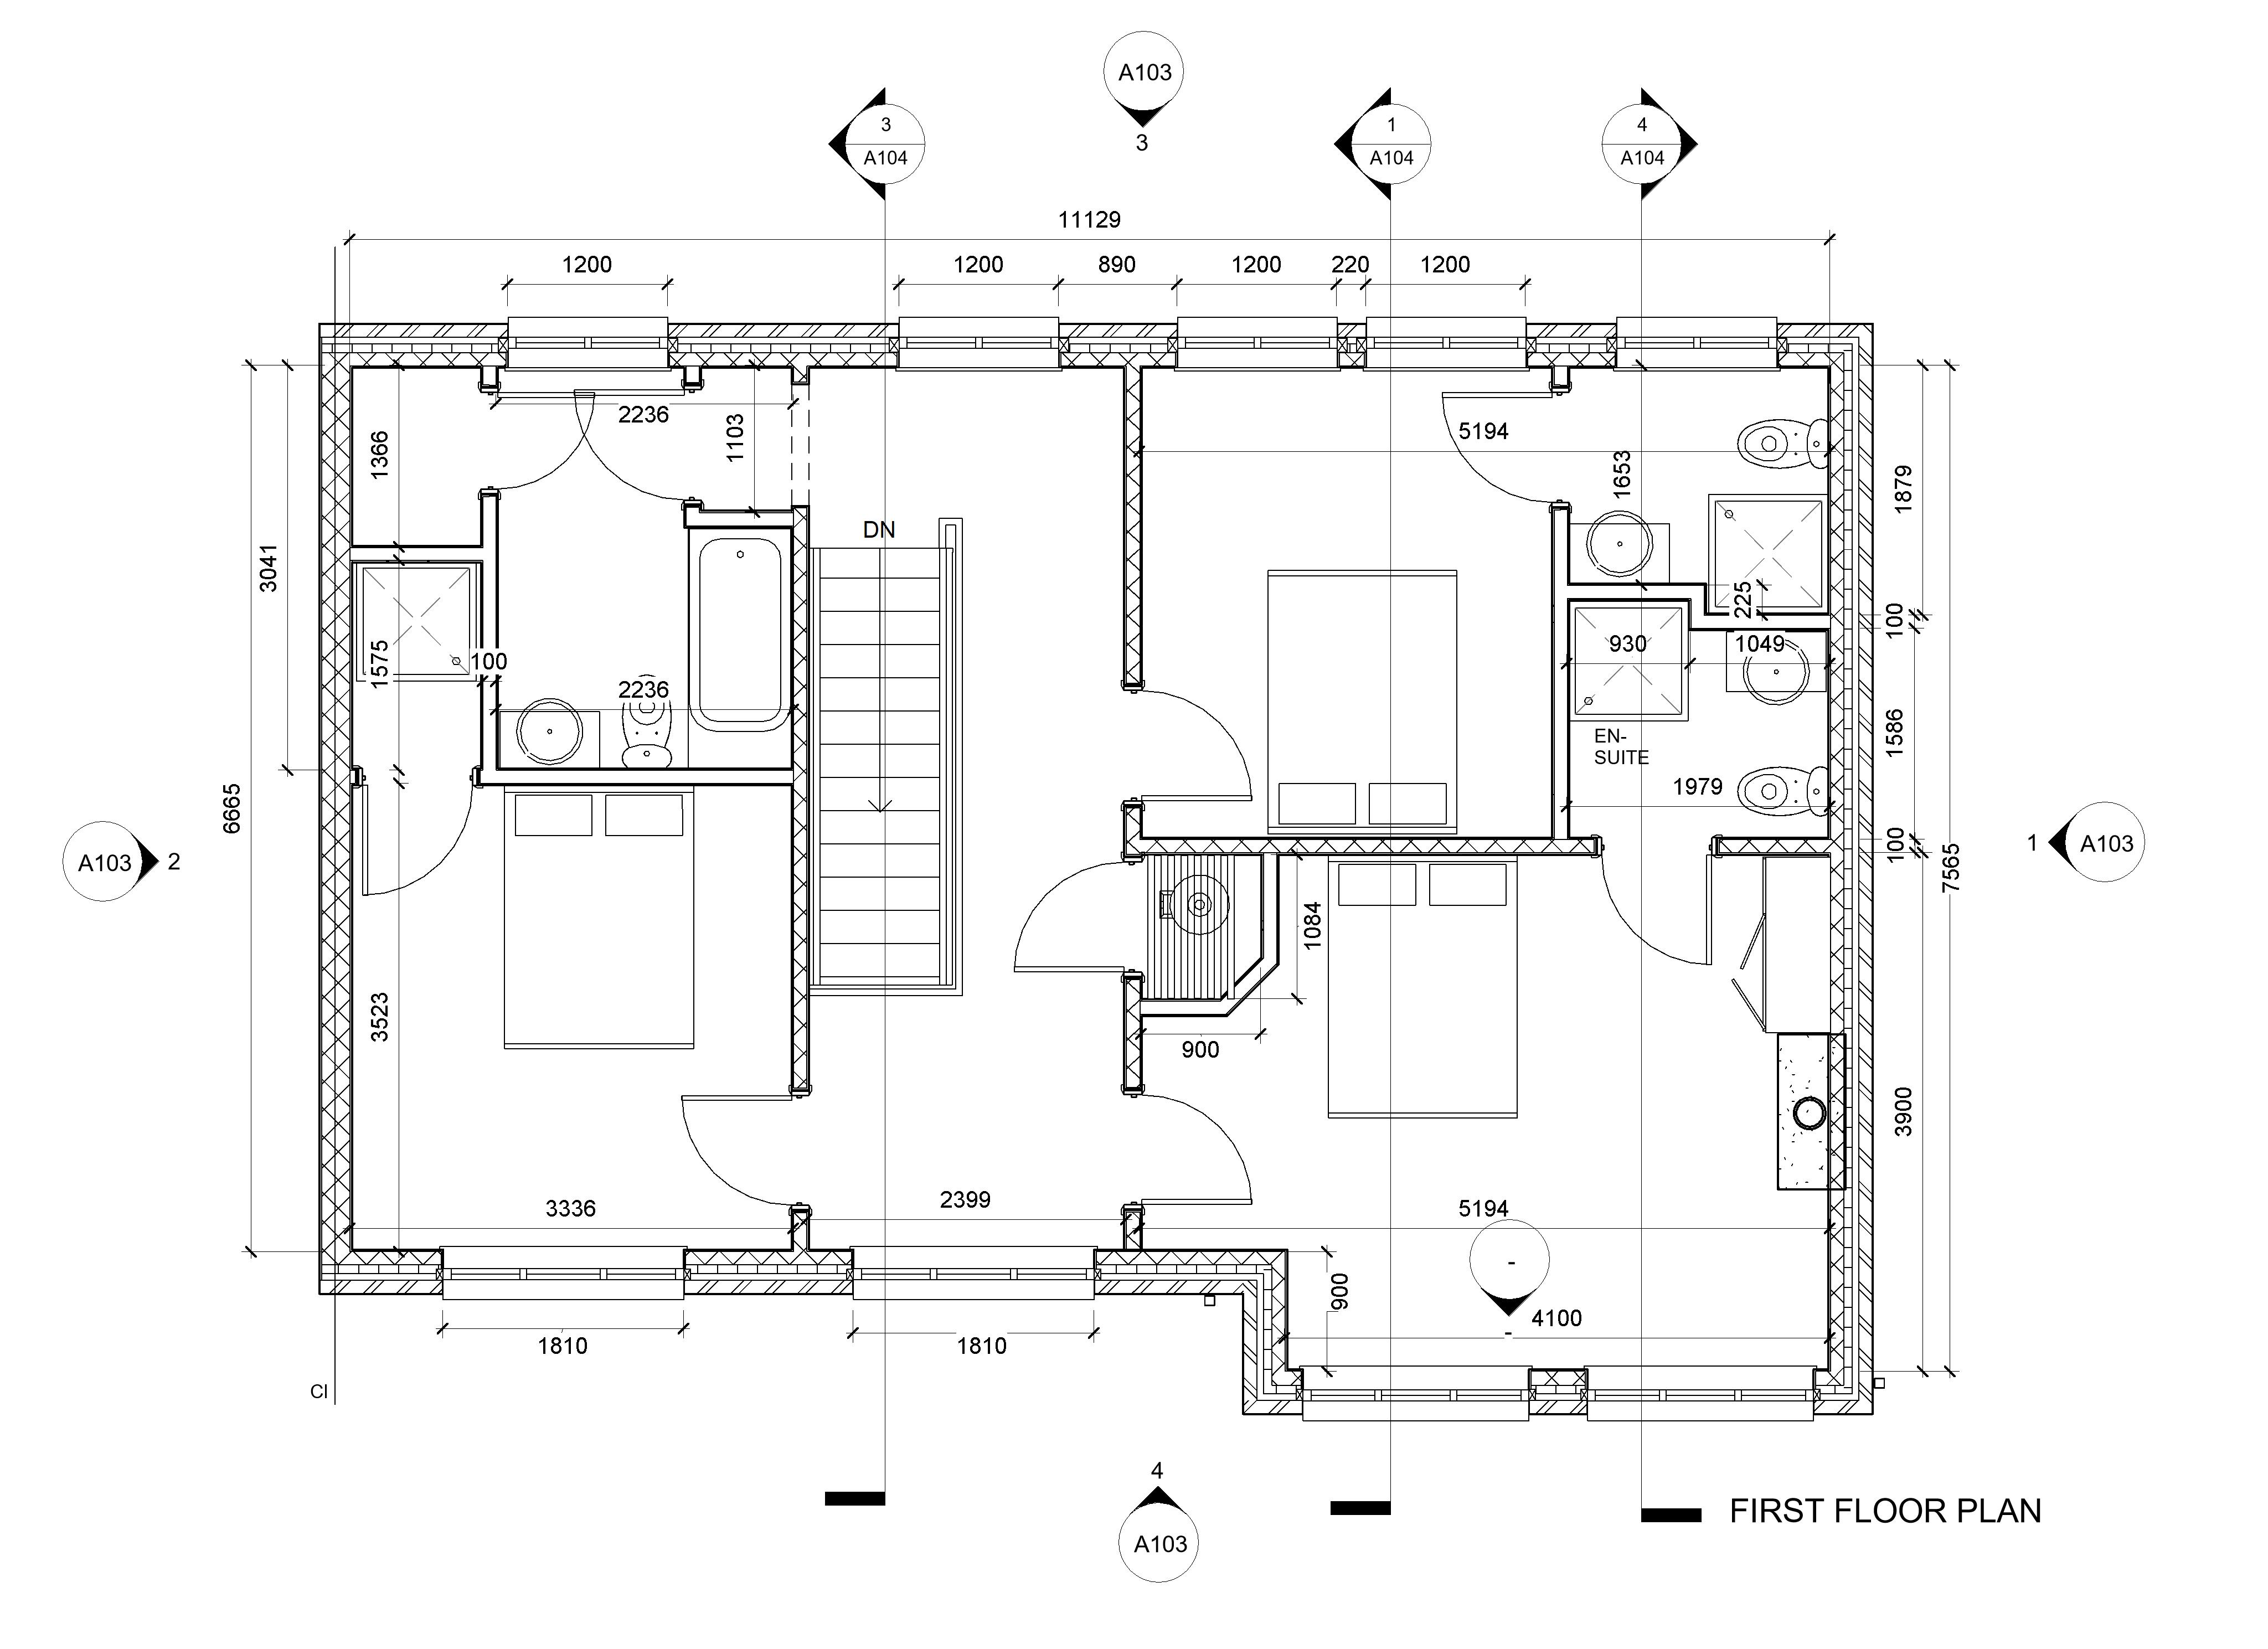
\includegraphics[width=1.0\linewidth]{img/P01FirstFloorLevel.jpg}
	\caption{First Floor Plan}
	\label{fig:p01firstfloorlevel}
\end{figure}


\newpage

\section*{Construction Specification}


\textbf{External Wall Specification} 

External walls are to be twin leaf cavity construction and be of a 4 part Stacked Wall Type
Wall-Ext-Stacked\_317 (4-Part-Dom) with the following layers

\begin{enumerate}
	\item L1\_Wall-Ext-Cav\_102Bwk-50Air-65Ins-100DBlk-15Rnd\&P (Gen Dom)
	\begin{itemize}
		\item Layer 1 (TopLayer) 'Variable'
		\item (315mm wide insulated Cavity Walls over DPC level - Generally)
		\item Made up of 102.5mm Brick / 50mm Air-gap / 65mm Insulation / 100mm Blockwork inner leaf
		\item Internal Finish 15mm (total) Render and Plaster
	\end{itemize}
	
	\item L2\_Wall-Ext\_CAv\_15Rnd-100Blk-50Air-65Ins-100DBlk-25Ins (Plinth)
	\begin{itemize}
		\item Layer 2 (Intermediate Layer) 225mm high
		\item (315mm wide insulated Cavity Wall at Plinth level)
		\item 15mm Cement Render (Plinth) / 100mm block / 50mm Air-gap / 65mm Insulation / 100mm Block
		\item 25mm thick perimeter insulation up-stand to internal face
	\end{itemize}
	
	
	\item L3\_Wall-Ext-Cav\_100Blk-115Conc-100DBlk (Rising Wall)
	\begin{itemize}
		\item Layer 3 (Intermediate Layer) 225mm high
		\item (315mm wide un-insulated Rising Wall)
		\item 100mm Block / 115mm wide Concrete filled cavity / 100mm Block inner leaf
	\end{itemize}
	
	
	\item L4\_Wall-Solid-440\_Trench-Blk
	\begin{itemize}
		\item Layer 4 (Base Layer) 675mm high
		\item (440mm wide Solid Trench Blockwork)
	\end{itemize}
\end{enumerate}

Foundations (Footings)

\begin{itemize}
	\item 1350 wide x 450 deep strip foundation
	\item Top of Strip foundation to be 1050mm below Gr. Floor level
\end{itemize}
1350 wide x 450 deep strip foundation


\subsection*{Internal Wall Specification}

\begin{itemize}
	\item Ground Floor Internal Walls
		\begin{itemize}
			\item Generally, Single leaf 100mm concrete block walls 15mm render / plaster both sides, (Wall-Part\_15Rnd\&P-100Blk-15Rnd\&P)
		\end{itemize}
	\item First Floor Internal Walls
		\begin{itemize}
			\item Landing Area: Single leaf 100mm concrete block walls, 15mm render / plaster both sides (Wall-Part\_15Rnd\&P-100Blk-15Rnd\&P)
			\item Elsewhere: 100mm timber stud partition, 15mm plaster slab / plaster both sides (Wall-Stud-Part\_15Gwb\&P-100Stud-15Gwb\&P) 
		\end{itemize} 
\end{itemize}



\subsection*{Floor Specification}


\begin{itemize}
	\item Ground Floor: Revit Library modified floor type (Floor-Grnd-Bearing) to be duplicated and used(Floor-Grnd-Bearing\_65Scr-100Ins-150Conc-DPM-50SBld-200Hcore)
	\begin{itemize}
		\item 65mm Sand \& Cement Screed on
		\item 100mm Floor Insulation on
		\item 150mm Reinforced Concrete Slab on
		\item Damp Proof Membrane on
		\item 50mm Sand Blinding on 
		\item 200mm Selected and Graded Hardcore laid in 2 No. 100mm layers
	\end{itemize}
	\item First Floor: Revit Library modified floor type (Floor\_Timber\_25Cbd-225Joist) may be used: Finished First Floor Level to be 2750mm (GFL to FFL)

\end{itemize}












\subsection*{Windows and Doors}
\begin{itemize}
	\item Head height - 2100mm
	\item Revit Library standard door types may be used
	\item External Front Door: Decorative type (panelled door with glazed side panels)
	\item External Kitchen and Boiler house doors to have glazed panels
	\item Generally, internal single doors to be standard flush-panel or regency panelled type
	\item Kitchen to living room doors to be double leaf, glazed multi-panel style
	\item Windows generally to be double or triple sash type with opening vents
	\item Dormer window: Rectangle or circular type as desired.
\end{itemize}






\subsection*{Electrical Fittings}
\begin{itemize}
	\item Kitchen and Living Room only, to be visible in Section or Camera View
	\item 2 No. Ceiling or Wall mounted light fittings per room
	\item 2 no. Twin Switched Socket power outlets per room
\end{itemize}





\subsection*{Ceilings}
\begin{itemize}
	\item 3mm Skim Coat Plaster on Gypsum Wall Board
	\item Revit Library 'modified' ceiling type (Compound Ceiling Plain)
	\item Ceiling Cut-outs required for Stairs and Dormer Window.
\end{itemize}



\subsection*{Roof Type}
\begin{itemize}
	\item Roof by Footprint
	\item Pitch 35\degree (also on Dormer)
	\item Main Roof overhang to be approx 300mm clear of outer leaf
	\item Dormer overhang to be approx 200mm clear of dormer walls
\end{itemize}



\subsection*{Roof Construction Specification}
\begin{itemize}
	\item Revit Library roof type 'Roof\_Pitched\_38Tile-25Bat-0Felt-25Bat-100Ins-150Truss-12PBd to be modified as follows: Roof\_Pitched\_38Tile-38Bat-0Feld-150Truss.
	\begin{itemize}
		\item 38mm Roofing Tile on 
		\item 38mm battens on 
		\item Roof Membrane on 
		\item 150mm Structure (Truss / Rafter)
	\end{itemize}
\end{itemize}




\subsection*{General Building}
Provide the following
\begin{itemize}
	\item Facia Boards, Flat Soffits, Rainwater Gutters, Downpipes and all necessary information to communicate design intent.
\end{itemize}


\subsection*{Site}
\begin{itemize}
	\item A basic flat topographical layer (Toposurface) is to be inserted in the Site View.  The toposurface be created at an elevation of -225mm
\end{itemize}


\end{document}